

%\documentclass{acm_proc_article-sp}
\documentclass{sig-alternate}
\usepackage{multirow}
\usepackage{fancyheadings}
\usepackage{algorithmic}
\usepackage{amssymb}
\usepackage{amsmath}
\usepackage{xspace}
\usepackage{pslatex}
\usepackage{microtype}
\usepackage{subfigure}
\usepackage{indentfirst}
\usepackage{listings, algorithm, algorithmic, graphicx, listing}
\usepackage{relsize}

%\usepackage{todonotes}
\usepackage{times}
\usepackage{graphicx}
\usepackage{epsf}
\usepackage{verbatim}
%\usepackage{psfig}
\usepackage{cite}
\usepackage{url}
\usepackage{color}
\usepackage{alltt}

\newcommand{\StateProjection}{static analysis}
\newcommand{\CurAspectJSubjectCount}{12}

\newcommand{\Add}{\CodeIn{add}}
\newcommand{\AVTree}{\CodeIn{AVTree}}
\newcommand{\Assignment}[3]{$\langle$ \Object{#1}, \Object{#2}, \Object{#3} $\rangle$}
\newcommand{\BinaryTreeRemove}{\CodeIn{BinaryTree\_remove}}
\newcommand{\BinaryTree}{\CodeIn{BinaryTree}}
\newcommand{\Caption}{\caption}
\newcommand{\Char}[1]{`#1'}
\newcommand{\CheckRep}{\CodeIn{checkRep}}
\newcommand{\ClassC}{\CodeIn{C}}
\newcommand{\CodeIn}[1]{{\small\texttt{#1}}}
\newcommand{\CodeOutSize}{\scriptsize}
\newcommand{\Comment}[1]{}
\newcommand{\Ensures}{\CodeIn{ensures}}
\newcommand{\ExtractMax}{\CodeIn{extractMax}}
\newcommand{\FAL}{field-ordering}
\newcommand{\FALs}{field-orderings}
\newcommand{\Fact}{observation}
\newcommand{\Get}{\CodeIn{get}}
\newcommand{\HashSet}{\CodeIn{HashSet}}
\newcommand{\HeapArray}{\CodeIn{HeapArray}}
\newcommand{\Intro}[1]{\emph{#1}}
\newcommand{\Invariant}{\CodeIn{invariant}}
\newcommand{\JUC}{\CodeIn{java.\-util.\-Collections}}
\newcommand{\JUS}{\CodeIn{java.\-util.\-Set}}
\newcommand{\JUTM}{\CodeIn{java.\-util.\-TreeMap}}
\newcommand{\JUTS}{\CodeIn{java.\-util.\-TreeSet}}
\newcommand{\JUV}{\CodeIn{java.\-util.\-Vector}}
\newcommand{\JMLPlusJUnit}{JML+JUnit}
\newcommand{\Korat}{Korat}
\newcommand{\Left}{\CodeIn{left}}
\newcommand{\Lookup}{\CodeIn{lookup}}
\newcommand{\MethM}{\CodeIn{m}}
\newcommand{\Node}[1]{\CodeIn{N}$_#1$}
\newcommand{\Null}{\CodeIn{null}}
\newcommand{\Object}[1]{\CodeIn{o}\ensuremath{_#1}}
\newcommand{\PostM}{\MethM$_{post}$}
\newcommand{\PreM}{\MethM$_{pre}$}
\newcommand{\Put}{\CodeIn{put}}
\newcommand{\Remove}{\CodeIn{remove}}
\newcommand{\RepOk}{\CodeIn{repOk}}
\newcommand{\Requires}{\CodeIn{requires}}
\newcommand{\Reverse}{\CodeIn{reverse}}
\newcommand{\Right}{\CodeIn{right}}
\newcommand{\Root}{\CodeIn{root}}
\newcommand{\Set}{\CodeIn{set}}
\newcommand{\State}[1]{2^{#1}}
\newcommand{\TestEra}{TestEra}
\newcommand{\TreeMap}{\CodeIn{TreeMap}}

\newenvironment{CodeOut}{\begin{scriptsize}}{\end{scriptsize}}
\newenvironment{SmallOut}{\begin{small}}{\end{small}}

\newcommand{\pairwiseEquals}{PairwiseEquals}
\newcommand{\monitorEquals}{MonitorEquals}
%\newcommand{\monitorWField}{WholeStateW}
\newcommand{\traverseField}{WholeState}
\newcommand{\monitorSMSeq}{ModifyingSeq}
\newcommand{\monitorSeq}{WholeSeq}

\newcommand{\IntStack}{\CodeIn{IntStack}}
\newcommand{\UBStack}{\CodeIn{UBStack}}
\newcommand{\BSet}{\CodeIn{BSet}}
\newcommand{\BBag}{\CodeIn{BBag}}
\newcommand{\ShoppingCart}{\CodeIn{ShoppingCart}}
\newcommand{\BankAccount}{\CodeIn{BankAccount}}
\newcommand{\BinarySearchTree}{\CodeIn{BinarySearchTree}}
\newcommand{\LinkedList}{\CodeIn{LinkedList}}

\newcommand{\Book}{\CodeIn{Book}}
\newcommand{\Library}{\CodeIn{Library}}

\newcommand{\Jtest}{Jtest}
\newcommand{\JCrasher}{JCrasher}
\newcommand{\Daikon}{Daikon}
\newcommand{\JUnit}{JUnit}

\newcommand{\trie}{trie}

\newcommand{\Perl}{Perl}


\newcommand{\SubjectCount}{11}
\newcommand{\DSSubjectCount}{two}

\newcommand{\Equals}{\CodeIn{equals}}
\newcommand{\Pairwise}{PairwiseEquals}
\newcommand{\Subgraph}{MonitorEquals}
\newcommand{\Concrete}{WholeState}
\newcommand{\ModSeq}{ModifyingSeq}
\newcommand{\Seq}{WholeSeq}
\newcommand{\Aeq}{equality}

\newcommand{\Meaning}[1]{\ensuremath{[\![}#1\ensuremath{]\!]}}
\newcommand{\Pair}[2]{\ensuremath{\langle #1, #2 \rangle}}
\newcommand{\Triple}[3]{\ensuremath{\langle #1, #2, #3 \rangle}}
\newcommand{\SetSuch}[2]{\ensuremath{\{ #1 | #2 \}}}
%\Comment{
%\newtheorem{definition}{Definition}
%\newtheorem{theorem}[definition]{Theorem}
%}
\newcommand{\Equiv}[2]{\ensuremath{#1 \EquivSTRel{} #2}}
\newcommand{\EquivME}{\Equiv}
\newcommand{\EquivST}{\Equiv}
\newcommand{\EquivSTRel}{\ensuremath{\cong}}
\newcommand{\Redundant}[2]{\ensuremath{#1 \lhd #2}}
\newcommand{\VB}{\ensuremath{\mid}}
\newcommand{\MES}{method-entry state}

\newcommand{\Small}[1]{{\small{#1}}}

\newcommand{\CenterCell}[1]{\multicolumn{1}{c|}{#1}}
\newcommand{\Fix}[1]{{\large\textbf{FIX}}#1{\large\textbf{FIX}}}

\newcommand{\CodeInS}[1]{{\scriptsize\texttt{#1}}}
\newcommand{\CodeInFN}[1]{{\footnotesize\texttt{#1}}}
\newcommand{\CodeOutFN}{\footnotesize}

\newcommand{\SmallSpace}{\vspace*{-1.4ex}}
\newcommand{\Item}{\SmallSpace\item}
\newenvironment{Itemize}{\begin{itemize}}{\end{itemize}\SmallSpace}
\newenvironment{Enumerate}{\begin{enumerate}}{\end{enumerate}\SmallSpace}

\newtheorem{definition}{Definition}
\newtheorem{theorem}[definition]{Theorem}

%\newcommand{\Item}{\vspace*{-0.5ex}\item\vspace*{-0.5ex}}
%\newenvironment{Itemize}{\begin{itemize}\vspace*{-1ex}}{\end{itemize}\vspace*{-1ex}}
%\newenvironment{Enumerate}{\begin{enumerate}\vspace*{-1ex}}{\end{enumerate}\vspace*{-1ex}}
\newenvironment{Definition}{\begin{definition}\vspace*{-1.5ex}}{\end{definition}\vspace*{-1.5ex}}

% Local Variables:
% mode:latex
% End:


% % Add line between figure and text
 \makeatletter
 \def\topfigrule{\kern3\p@ \hrule \kern -3.4\p@} % the \hrule is .4pt high
 \def\botfigrule{\kern-3\p@ \hrule \kern 2.6\p@} % the \hrule is .4pt high
 \def\dblfigrule{\kern3\p@ \hrule \kern -3.4\p@} % the \hrule is .4pt high
 \makeatother

 % If there is a line, you can get away with reducing the separation between
 % figures and text.  Don't do this without the line, though.
 \addtolength{\textfloatsep}{-.5\textfloatsep}
 \addtolength{\dbltextfloatsep}{-.5\dbltextfloatsep}
 \addtolength{\floatsep}{-.5\floatsep}
 \addtolength{\dblfloatsep}{-.5\dblfloatsep}

% Left and right curly braces in tt font
\newcommand{\ttlcb}{\texttt{\char "7B}}
\newcommand{\ttrcb}{\texttt{\char "7D}}

\newcommand{\totaloc}{99458 }
\newcommand{\subnum}{10 }
\newcommand{\warnings}{22 }
\newcommand{\bugs}{12 }
\newcommand{\newbugs}{7 }
\newcommand{\falses}{10 }
\newcommand{\annotationnum}{7 }
\newcommand{\filternum}{11 }

% \newcommand{\smallstep}{\vspace{-2mm}}
% \newcommand{\tinystep}{\vspace{-1mm}}
\newcommand{\smallstep}{\relax}
\newcommand{\tinystep}{\relax}


\newenvironment{myindentpar}[1]%
{\begin{list}{}%
         {\setlength{\leftmargin}{#1}}%
         \item[]%
}
{\end{list}}


% Reduce indentation in lists.
%\setlength{\leftmargini}{.5\leftmargini}

%% Bring items closer together in list environments
%% This doesn't work with an optional argument to the list environment.
% Prevent infinite loops
\let\Itemize =\itemize    
\let\Enumerate =\enumerate
\let\Description =\description
% Zero the vertical spacing parameters
\def\Nospacing{\itemsep=0pt\topsep=0pt\partopsep=0pt\parskip=0pt\parsep=0pt}
% Redefine the environments in terms of the original values
\renewenvironment{itemize}{\Itemize\Nospacing}{\endlist}
\renewenvironment{enumerate}{\Enumerate\Nospacing}{\endlist}
\renewenvironment{description}{\Description\Nospacing}{\endlist}

\newcommand{\todo}[1]{{TODO #1}}
\newcommand{\sai}[1]{{\color{blue}\todo{for Sai: #1}}}
\newcommand{\yuyin}[1]{{\color{red}\todo{for Yuyin: #1}}}

\begin{document}

\title{Synthesizing SQL Queries from Input-Output Examples}
%\subtitle{[CSE 544, Course Project Milestone Report, Spring 2012]}
%\titlenote{This work is sponsored by}


\author{
\alignauthor Sai Zhang \quad Yuyin Sun\\
       \affaddr{Department of Computer Science \& Engineering}\\
       %\affaddr{1932 Wallamaloo Lane}\\
       \affaddr{University of Washington}\\
       \email{\{szhang, sunyuyin\}@cs.washington.edu}
}


\maketitle

\begin{abstract}

In the age of big data, a large number of computer end-users, such as
research scientists and business analysts, need to frequently query
a database, yet lack the programming knowledge to do such tasks smoothly.
In this paper, we present a \textit{programming by example} technique
that permits end-users to automate such querying tasks.
Our technique takes from users an input and output example of how the
database should be queried, and synthesizes a SQL query that
reproduces the example output from the example input. Later, when the synthesized
SQL query is applied to another, potentially larger, database with a
similar schema as the example input, the synthesized SQL query produces
a corresponding result that is similar to the example output. Our technique
has several notable features: it only needs small input-output examples
to infer a desirable SQL query, it is fully automated and does not require
users to provide annotations/hints of any form, and it can rank multiple
possible solutions to provide to users the most likely result.


Our technique has been implemented as an open-source programming
tool. In our preliminary evaluation, our prototype tool has synthesized correct
answers for 5 out of 6 SQL exercises from a classic database textbook,
and has been used to solve 5 non-trivial problems raised by real-world
users from popular online forums, including ones that receive no human replies.

%This opens up an amazing
%set of possibilities in the context of making classroom teaching
%interactive


\end{abstract}


\section{Introduction}
\label{sec:introduction}


The big data revolution over the past few years has resulted
in significant advances in digitization of massive amounts
of data and accessibility of computational devices to massive
proportions of the population. A perennial challenge faced by many
enterprise nowadays is the management
of their increasingly large and complex databases, which can contain
hundreds and even thousands of tables. 


%but they often need to
%query databases to obtain relevant data to support their business decisions.


\subsection{End-users' Difficulties in Using SQL}
Although the relational database management system (RDBMS) and the
de facto language (SQL) are perfectly adequate for many end-users'
needs~\cite{Howe:2011}, the costs associated with deployment and
use of database software and SQL are prohibitive. 

The problem is exacerbated by the fact that many end-users
have myriad diverse backgrounds including research scientists,
business analysts, commodity traders, human resource managers,
finance professionals, and marketing managers. Increasingly,
those end-users who need to query databases to analyze the
data are not professional programmers, but are experts in some
other domains. They need to ask a variety of questions on their
data and use the answer to support their business decisions.
For example, as pointed out
by~\cite{Gray:2005}, conventional RDBMS software remains underused
in the long tail of science: the large number of users, such as the
research scientists who are in relatively small labs and individual
researchers, have limited IT funding, staff and infrastructure yet
collectively produce the bulk of scientific knowledge. 

%Similarly, other end-users
%such as business analysts who query databases frequently often
%do not have significant SQL expertise.

For a large number of end-users, they learn and use SQL queries in
the following typical ways: they browse textbook or online resources to learn basic
idioms of SQL. They try to write experimental SQL queries and execute them
on sample databases to explore the data itself. They modify
the written queries to derive new queries by adding or removing snippets:
predicates in the \CodeIn{where} clause,
tables in the \CodeIn{from} clause, or columns in the \CodeIn{select} clauses.
However, such practice is inefficient and time-consuming.
A key challenge is that many end-users can clearly understand
their goals but simply can not write a correct SQL query for
their tasks, either due to the syntax complexity of the language itself,
or the structure complexity of the underlying databases, or others.
For many end-users, they need an \textit{intelligent} tool
to assist them to perform database query tasks. A highly accessible tool
that end-users can describe their needs, and use to connect their
intentions to executable
SQL queries would be best.


\subsection{Existing Solutions}


\textit{Graphical User Interface} (GUI) and \textit{general programming languages}
are two state-of-the-art approaches in helping end-users perform
database queries. However, both of them are far from satisfactory.

Many RDBMS come with a well-designed GUI with tons of features.
However, 
%as a database management system often comes with tons
%of features, end-users struggle to find the correct feature or
%succession of commands to use from a maze of features to accomplish
%their tasks.
a GUI often does not permit users to personalize
a database's functionality for user-specific tasks. On the other hand,
as a GUI supports more and more customization features, users
may struggle to discover those features, which can significantly
degrade its usability. 

General programming languages, such as SQL,
Java (with JDBC), or other domain specific languages, 
serve as a fully expressive medium  for
communicating a user's intention to a database. However, learning
a practical programming language (even a simplified, high-level domain
specific language) often requires a substantial amount
of time and energy that a typical end-user would not prefer,
and should not be expected, to invest. 



\subsection{Synthesizing SQL Queries from Examples}

After carefully studying how end-users were describing their
encountered SQL query problems on online help forums, we observed that
one of the most common ways for end-users to
express their intents is using input-output examples. Although
input-output examples may lead to underspecification, they
serve as a straightforward way of describing \textit{what} the
task is and a natural interface that a tool can provide assistance.


In this work, we present a technique for synthesizing SQL queries
from input-output examples. In particular, our technique takes example input
table(s) and output table from the end-users, and then automatically
infers a SQL query (or multiple queries, if exist) that queries
the input database and returns the output example. If the inferred
SQL query is applied
to the example input, then it produces the example output, and if the
SQL query is applied to other similar inputs (potentially much larger tables),
then the SQL query produces a corresponding output.

Our technique follows a general methodology for designing
systems supporting programming by examples~\cite{Harris:2011}.
It includes the following three major steps:
(1) identify a language subset (of SQL) that is expressive to
describe a large proportion of %operations that users need to perform
database queries; (2) design an algorithm that
can efficiently infer programs in the language from input-output
examples; and (3) develop a ranking strategy that presents
the most likely program to the users, when multiple solutions exist.

\vspace{1mm}
\noindent \textbf{\textit{Supported SQL Subset.}}
The full SQL 93 specification contains over 1000 pages, and it is
infeasible and unnecessary to support all language features in practice.
When selecting a supported SQL subset, there is a tradeoff
between the expressiveness of the selected language subset,
and the complexity of finding simple consistent solutions
within that language's search space.  In general, the more expressive a search
space, the harder the task of finding consistent hypotheses within
that search space. 

During our study of end-user's real problems, we also carefully studied what would
be the solution to users' desired query, and found that the most common
desired queries can be composed by a handful of basic SQL constructs,
which form the target language of this work (Section~\ref{sec:langsubset}).

As shown in our experiments (Section~\ref{sec:evaluation}), the supported subset, though far from completion, is expressive
enough to describe many query tasks succinctly, while at the same time concise
enough to be amenable for efficient inference. 



\vspace{1mm}
\noindent \textbf{\textit{SQL Query Inference Algorithm.}} Our inference
algorithm, as described in Section~\ref{sec:approach}, consists of two
major steps. The first step, called \textit{SQL Skeleton Creation}, scans
the example input and output, and \textit{guesses} what a desirable
SQL query may look like. The output of this step is a set of \textit{incomplete} SQL
query skeletons. A SQL query skeleton is an incomplete SQL query,
which contains unknown parts. The second step,
called \textit{SQL Query Completion} takes as inputs a created
SQL skeleton, fills unknown parts with possible solutions, and then produces a set of
syntactically-valid SQL queries. In particular, when performing
SQL query completion, our technique uses a rule learning algorithm
to infer the conditions (Section~\ref{sec:decision_tree}), and uses 
type-directed search to infer possible aggregates in a query (Section~\ref{sec:agg_search}).

\vspace{1mm}
\noindent \textbf{\textit{Query Candidate Ranking Strategy.}}
Input-output examples provided by end-users are likely to
be under-specified. It is entirely possible that multiple
queries can be synthesized to satisfy the provided examples.
We address this problem by developing a ranking scheme that 
ranks the possibly multiple queries
consistent with the given input-output
examples. Our ranking scheme, detailed in Section~\ref{sec:ranking}
is inspired by the Occam's razor principle, prefers a smaller and
simpler solution if other aspects being equal.

%is usually the correct one. 

%Besides
%selecting a smaller one, we could also compute the likelihood
%of each query being correct based on some statistics, and then
%pick the most likely one.


\subsection{Technique Evaluation}

The goal of this work is developing a practical SQL query synthesis technique that is capable of
helping end-users writing a wide range of SQL queries.
The technique aims to replace the role of the forum expert,
which not only removes human from the loop, but also enables
end-users to solve their problems in a few seconds as opposed to a few days
(while waiting for an expert's reply). 

Thus, we implemented our technique in an open-source tool
and evaluated it in two ways. First, we picked up 6 SQL
exercises from a classic database textbook~\cite{cowbook}. SQL exercises
from a database textbook often cover
the most widely-used SQL features 
that a course instructor wishes students to master.
Those exercises can be served as golden test
to evaluate the expressiveness of our supported SQL subset. Second,
we collected 5 non-trivial SQL problems raised by real end-users on online
help forums, and tested whether our technique can effectively synthesize desirable
SQL queries.

As a result, our technique successfully synthesized 5 out of 6
textbook exercises and solved all 5 forum problems, within a very
small amount of time (1 minute per exercise/problem, on average).

\subsection{Contributions}

This paper makes the following contributions:

\begin{itemize}
\item \textbf{Problem.} To the best of our knowledge, we are the first
to address the SQL query synthesis problem from examples across multiple
tables.
%An approach to automatically synthesizing SQL
%queries from input-output examples (Section~\ref{sec:approach}).

\item \textbf{Technique.} We show to automatically synthesize SQL
queries from input-output examples (Section~\ref{sec:approach}).

\item \textbf{Tool.} A practical tool that implements the proposed technique (available at:
\url{http://sqlsynthesizer.googlecode.com}).

\item \textbf{Evaluation.} An empirical evaluation of the tool implementation
on a number of SQL exercises from a classic textbook~\cite{cowbook}
and SQL problems raised by real users on online forums (Section~\ref{sec:evaluation}).
\end{itemize}


%%\section{A Motivating Example}
%\label{sec:example}

Consider the following SQL question picked up from a classic
database textbook~\cite{cowbook}: \textit{given a \CodeIn{student} table (Figure~\ref{tbl:student})
and an \CodeIn{enrolled} table (Figure~\ref{tbl:enrolled}), find out the name and max score of the
students whose level is senior and enrolled in more than 3 courses}.



\begin{figure}[t]
	\centering
\begin{tabular}{|c|c|c|}
\hline
 Student\_key& Student\_name & Level\\
\hline
 0001 & Adam & senior \\
 \hline
 0002 & Bob & junior \\
 \hline
 0003 & Erin & senior \\
 \hline
 0004 & Rob & junior\\
 \hline
 0005 & Dan & senior \\
 \hline
 0006 & Peter & senior \\
 \hline
 0007 & Sai & senior \\
 \hline
\end{tabular}
	\caption{An example input table `student'
for the SQL question described in
Section~\ref{sec:example}.}
	\label{tbl:student}
\end{figure}


\begin{figure}[t]
	\centering
\begin{tabular}{|c|c|c|}
\hline
 Student\_key& Course\_key& Score \\
\hline
 0001 & 001 & 4 \\
\hline
 0001 & 002 & 2 \\
\hline
 0002 & 001 & 3 \\
\hline
 0002 & 002 & 2 \\
\hline
 0002 & 003 & 3 \\
\hline
 0003 & 002 & 1 \\
\hline
 0004 & 001 & 4 \\
\hline
 0004 & 003 & 4 \\
\hline
 0005 & 002 & 5 \\
\hline
 0005 & 003 & 2 \\
\hline
 0005 & 004 & 1 \\
\hline
 0006 & 002 & 4 \\
\hline
 0006 & 004 & 5 \\
\hline
 0007 & 001 & 2 \\
\hline
 0007 & 003 & 3 \\
\hline
 0007 & 004 & 4 \\
 \hline
\end{tabular}
	\caption{An example input table  `enrolled'
for the SQL question described in
Section~\ref{sec:example}.}
	\label{tbl:enrolled}
\end{figure}	

\begin{figure}[t]
	\centering
\begin{tabular}{|c|c|}
\hline
 Student\_name & Max\_score \\
\hline
 Dan & 5 \\
\hline
 Sai & 5 \\
 \hline
\end{tabular}
	\caption{An example output table for the SQL question described in
Section~\ref{sec:example}.}
	\label{tbl:output}
\vspace{3mm}
\end{figure}		


\begin{figure}[t]
\begin{CodeOut}
\begin{alltt}
\textbf{select student.Student\_name, max(enrolled.Score)
from student, enrolled
where student.Student\_key = enrolled.Student\_key
      and student.Level = `senior'
group by student.Student\_key
having count(enrolled.Course\_key) > 3}
\end{alltt}
\end{CodeOut}
\vspace{-5mm}
	\caption{A SQL query to solve the SQL question described in
Section~\ref{sec:example}. When applied to the input tables in
Figure~\ref{tbl:student} and Figure~\ref{tbl:enrolled}, it produces the result table
in Figure~\ref{tbl:output}.}
	\label{fig:expected_sql}
\end{figure}

The question's description is quite simple.
For a novice user, although they have a clear
intention of what the query should do, the answer (Figure~\ref{fig:expected_sql}) may
not be that straightforward. 

Despite the possible difficult in writing a correct SQL query,
a user could still easily draw
two input tables (Figure~\ref{tbl:student} and Figure~\ref{tbl:enrolled})
and one output table (Figure~\ref{tbl:output}) that fulfill the
SQL question.

In the \CodeIn{student} table, column {\CodeIn{Student\_key}} with
\CodeIn{String} type serves as the primary key. 
%Columns {\CodeIn{Student\_name}} and {\CodeIn{Level}} are \textsf{String}-type.
In the \CodeIn{enrolled} table, both columns {\CodeIn{Student\_key}} and
{\CodeIn{Course\_key}} are two foreign keys, and column {\CodeIn{Score}}
with \CodeIn{Integer} type keeps students' scores on their enrolled courses.

In the output table, the first column  {\CodeIn{Student\_name}}
comes from table \textit{student}, and the second column {\CodeIn{Max\_score}}
is a aggregation attribute.% summarizing the with type of \CodeIn{Integer}.

Having the input and output examples, our technique successfully synthesizes
the desirable SQL query as shown in Figure~\ref{fig:expected_sql}.


\newcommand{\q}{\langle query\rangle}
\newcommand{\db}{\langle db\rangle}
\newcommand{\pat}{\langle pat\rangle}
\newcommand{\bug}{\langle bug\rangle}
\newcommand{\dist}{\langle distance\rangle}
\newcommand{\sem}[1]{\llbracket #1\rrbracket}
\newcommand{\lit}[1]{\texttt{#1}}

\newcommand{\column}{\langle column\rangle}
\newcommand{\dbtable}{\langle table\rangle}
\newcommand{\cond}{\langle cond\rangle}
\newcommand{\op}{\langle op\rangle}
\newcommand{\e}{\langle expr\rangle}
\newcommand{\ce}{\langle cexpr\rangle}

\begin{figure}[t]
%\scriptsize{%
\footnotesize%
\begin{align*}
\q ::= {} 
	& \texttt{ SELECT } \e^+ \texttt{ FROM } \dbtable^+ \\
        & \texttt{ WHERE } \cond^+ \\ 
	&  \texttt{ GROUP BY } \column^+ \texttt{ HAVING } \cond^+\\
\dbtable::= {} &\ atom \\
\column ::= {} &\ \dbtable.atom\\
\cond ::= {} &\ \ \cond \;\texttt{\&\&}\; \cond \\ 
    & |\ \cond \;\texttt{||}\; \cond \\
    & |\ \texttt{(}\;\cond\;\texttt{)} \\
    & |\ \ce \;\op\; \ce \\
\op ::= {} &\ \ \texttt{=} \;\;|\;\; \texttt{>}  \;\;|\;\; \texttt{<}\\
\ce ::= {} &\ \ const \;\;|\;\; \column  \;\; \\
\e ::= {} & \ce \;\;|\ count(\column) \\
    & |\ sum(\column) \;\;|\ max(\column) \;\;|\ min(\column) 
\end{align*}
\normalsize%
\caption{Syntax of the supported SQL subset.}
\label{fig:syntax}
\end{figure}


\section{Language and Example}
\label{sec:langsubset}

In this section, we first present the supported SQL subset, and
then describe a motivating example which could be expressed in the
supported SQL subset.

\subsection{Supported SQL Subset}

Figure~\ref{fig:syntax} defines the syntax of the supported language,
which
is a subset of the standard SQL 93 language. This language subset
supports common query operations across multiple tables (i.e.,
\CodeIn{select} ... \CodeIn{from} ... \CodeIn{where}..), and 
conjunction of predicates. The language
subset shares the same semantics with the standard SQL language.
Differing from language subsets used in the
existing work~\cite{DasSarma:2010}, our language subset
supporting
joining operations across multiple tables, and includes
widely-used database operations such as \CodeIn{group by},
\CodeIn{order by}, and \CodeIn{having}, as
well as a few common aggregation functions such as \CodeIn{count}, \CodeIn{sum},
\CodeIn{max}, and \CodeIn{min}.

As we will show in Section~\ref{sec:evaluation}, this
subset, though far from completion, is expressive enough for answering
many evaluated SQL exercises from a textbook and some real problems
from online forums.

\subsection{Motivating Example}
\label{sec:example}

%\section{A Motivating Example}
%\label{sec:example}

Consider the following SQL question picked up from a classic
database textbook~\cite{cowbook}: \textit{given a \CodeIn{student} table (Figure~\ref{tbl:student})
and an \CodeIn{enrolled} table (Figure~\ref{tbl:enrolled}), find out the name and max score of the
students whose level is senior and enrolled in more than 3 courses}.



\begin{figure}[t]
	\centering
\begin{tabular}{|c|c|c|}
\hline
 Student\_key& Student\_name & Level\\
\hline
 0001 & Adam & senior \\
 \hline
 0002 & Bob & junior \\
 \hline
 0003 & Erin & senior \\
 \hline
 0004 & Rob & junior\\
 \hline
 0005 & Dan & senior \\
 \hline
 0006 & Peter & senior \\
 \hline
 0007 & Sai & senior \\
 \hline
\end{tabular}
	\caption{An example input table `student'
for the SQL question described in
Section~\ref{sec:example}.}
	\label{tbl:student}
\end{figure}


\begin{figure}[t]
	\centering
\begin{tabular}{|c|c|c|}
\hline
 Student\_key& Course\_key& Score \\
\hline
 0001 & 001 & 4 \\
\hline
 0001 & 002 & 2 \\
\hline
 0002 & 001 & 3 \\
\hline
 0002 & 002 & 2 \\
\hline
 0002 & 003 & 3 \\
\hline
 0003 & 002 & 1 \\
\hline
 0004 & 001 & 4 \\
\hline
 0004 & 003 & 4 \\
\hline
 0005 & 002 & 5 \\
\hline
 0005 & 003 & 2 \\
\hline
 0005 & 004 & 1 \\
\hline
 0006 & 002 & 4 \\
\hline
 0006 & 004 & 5 \\
\hline
 0007 & 001 & 2 \\
\hline
 0007 & 003 & 3 \\
\hline
 0007 & 004 & 4 \\
 \hline
\end{tabular}
	\caption{An example input table  `enrolled'
for the SQL question described in
Section~\ref{sec:example}.}
	\label{tbl:enrolled}
\end{figure}	

\begin{figure}[t]
	\centering
\begin{tabular}{|c|c|}
\hline
 Student\_name & Max\_score \\
\hline
 Dan & 5 \\
\hline
 Sai & 5 \\
 \hline
\end{tabular}
	\caption{An example output table for the SQL question described in
Section~\ref{sec:example}.}
	\label{tbl:output}
\vspace{3mm}
\end{figure}		


\begin{figure}[t]
\begin{CodeOut}
\begin{alltt}
\textbf{select student.Student\_name, max(enrolled.Score)
from student, enrolled
where student.Student\_key = enrolled.Student\_key
      and student.Level = `senior'
group by student.Student\_key
having count(enrolled.Course\_key) > 3}
\end{alltt}
\end{CodeOut}
\vspace{-5mm}
	\caption{A SQL query to solve the SQL question described in
Section~\ref{sec:example}. When applied to the input tables in
Figure~\ref{tbl:student} and Figure~\ref{tbl:enrolled}, it produces the result table
in Figure~\ref{tbl:output}.}
	\label{fig:expected_sql}
\end{figure}

The question's description is quite simple.
For a novice user, although they have a clear
intention of what the query should do, the answer (Figure~\ref{fig:expected_sql}) may
not be that straightforward. 

Despite the possible difficult in writing a correct SQL query,
a user could still easily draw
two input tables (Figure~\ref{tbl:student} and Figure~\ref{tbl:enrolled})
and one output table (Figure~\ref{tbl:output}) that fulfill the
SQL question.

In the \CodeIn{student} table, column {\CodeIn{Student\_key}} with
\CodeIn{String} type serves as the primary key. 
%Columns {\CodeIn{Student\_name}} and {\CodeIn{Level}} are \textsf{String}-type.
In the \CodeIn{enrolled} table, both columns {\CodeIn{Student\_key}} and
{\CodeIn{Course\_key}} are two foreign keys, and column {\CodeIn{Score}}
with \CodeIn{Integer} type keeps students' scores on their enrolled courses.

In the output table, the first column  {\CodeIn{Student\_name}}
comes from table \textit{student}, and the second column {\CodeIn{Max\_score}}
is a aggregation attribute.% summarizing the with type of \CodeIn{Integer}.

Having the input and output examples, our technique successfully synthesizes
the desirable SQL query as shown in Figure~\ref{fig:expected_sql}.




\section{Technique}
\label{sec:approach}



We next describe our SQL query synthesis technique in detail.
How to infer the desirable query for the examples
shown in Section~\ref{sec:example} will
be discussed thoroughly in this section.

\begin{figure}[t]
  \centering
  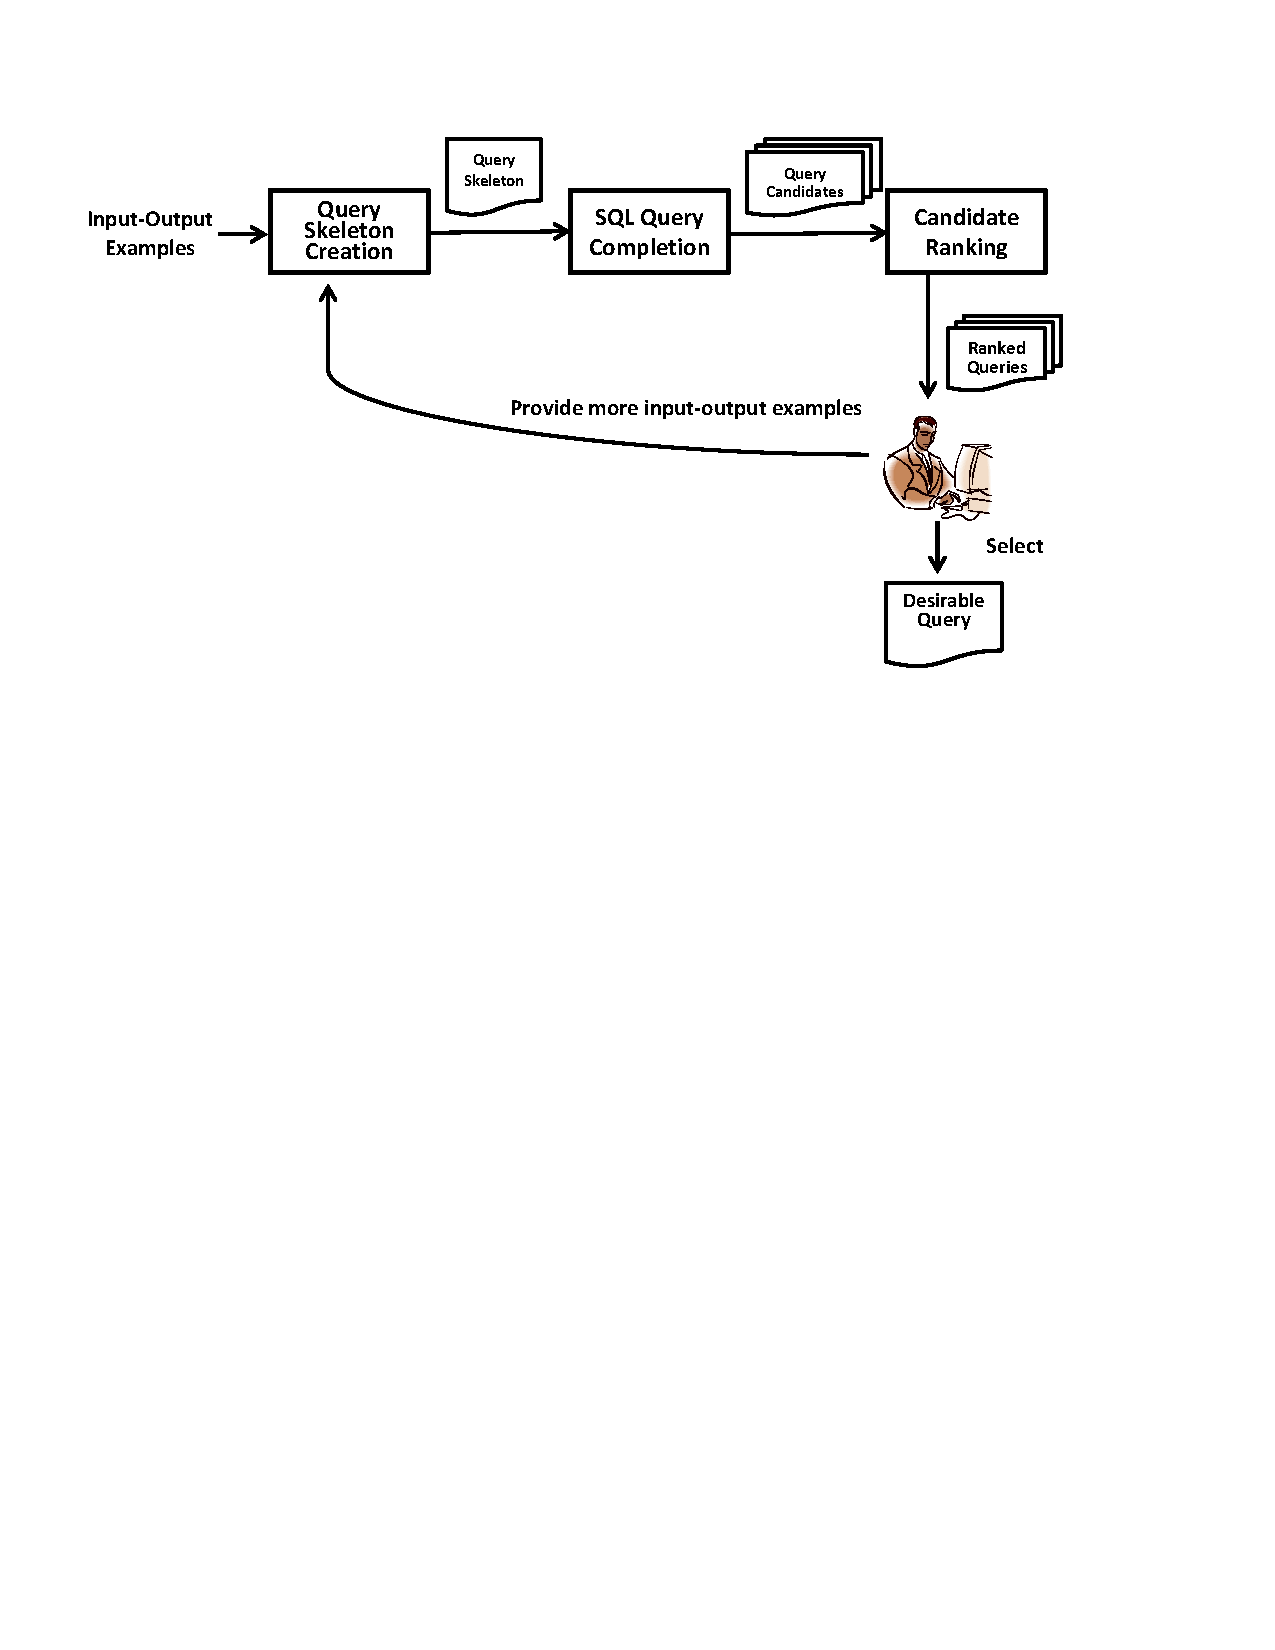
\includegraphics[scale=0.50]{workflow}
  \vspace*{-5.0ex}\caption {{\label{fig:workflow} The workflow of our SQL query synthesis approach.
}}

\end{figure}

\subsection{Overview}
Figure~\ref{fig:workflow} sketches the general workflow of our technique.
At a high level, our technique consists of three major steps: Query Skeleton
Creation(Section~\ref{sec:skeleton}), SQL Query Completion
(Section~\ref{sec:completion}), and Query Candidate Ranking (Section~\ref{sec:ranking}).
Specifically, our approach takes from users input-output examples. It first infers
a partially-complete query skeleton. The inferred query skeleton, though contains
incomplete parts that can not be yet decided, serves as a good reference
for further synthesizing a complete SQL query.
After that, our technique uses two techniques to complete a SQL skeleton.
In particular, it uses an advanced rule learning algorithm from the machine
learning community to infer query conditions (Section~\ref{sec:decision_tree}), and
 employs type-directed search to figure out possible aggregation
expressions (Section~\ref{sec:agg_search}).
The SQL Query Completion step produces a list of syntactically-valid
query candidates that satisfy the provided input-output examples.
However, it is possible that multiple query candidates can be synthesized based on the
provided input-output example. To deal with that, our technique
ranks all generated candidates,
and provides users a ranked list of SQL queries with the
simplest ones on the top. 
%This makes our tool more usable.


End-users can use our approach to obtain SQL query to transform
multiple, huge database tables by constructing small, representative
input and output example tables. On some examples, we speculate
that our approach
may produce a SQL query that satisfies the input and output examples
given by the user, but does not address the intention
that the user wants. To address this issue, we adapt a simple
interaction model from~\cite{Harris:2011} to ask users to investigate the results of
an output SQL query and report any discrepancy. In this case,
the user can refine the inferred SQL query by providing a more
informative input-output example (or multiple input-output examples
that together describe the required behavior) that demonstrate the behavior on
which the originally-inferred SQL query behaves incorrectly.

\subsection{Query Skeleton Creation}
\label{sec:skeleton}

In this step, our technique scans the provided input and output examples, guesses
what a target SQL query might look like, and infers a set of query skeletons
that capture the basic query structures.

A query skeleton is an incomplete SQL query, which
captures three basic query structures that could
often be decided after a simple scan over the examples:
tables used in a result SQL
query, table columns used to join input tables, and table
columns for projecting the query results. Other parts in a SQL query such as conditions
(including selection and having conditions), and aggregations
are left as unkown, and will be determinated in the next step (Section~\ref{sec:completion}).



%\begin{itemize}

%\item
\vspace{1mm}
\noindent \textit{\textbf{Step 1: Determining the Table Set.}} 
In practice, end-users are unwilling to provide more than enough
inputs. Therefore, every input table specified in the example
is expected to be used to construct a desirable SQL query.
Based on this observation, we assume that every input table
should be used as least once in the query. By default, the
table set $T$ used in the result SQL query contains all given input tables.
However, it is possible that a single table will be used for multiple times.
Our technique does not forbid this case, rather, we adopt a single heuristic
to estimate the used table set: if the same column from an input table appears more than once in the
example output, we add the input table the same number of times to the used table set.

%we view it as a strong indicator that this table will be joined multiple times and add it to our table
%set $T$ using an alias.


%\item
\vspace{1mm}
\noindent\textit{\textbf{Step 2: Determining Joining Columns. }} Given two arbitrary tables, there exist many
ways to join them. Enumerating all possible joining conditions may introduce a huge number of joining
conditions and would quickly become intractable. We observe that, in practice, two tables are often joined via the following
three cases: (1) tables are joined on their primary keys with the same (or compatible) data types, such
as joining a \textit{student} table with an \textit{enrolled} table with the \textit{student\_id} column. It does not
make any sense to join two tables on a Integer column and a String column; (2) tables are joined
using columns with the same name, such as joining a \textit{student} table with a \textit{enrolled} table on the
\textit{student\_name} column; and (3) two columns that have the data type, and have a large portion of
overlapped values in their corresponding input tables can be used as a joining condition. It is straightforward to check the first 
two cases to identify possible joining columns. For the third case, our technique scans the given input tables to check ``value similarity''
between two arbitrary columns, and selects columns whose ``value similarity'' is above a fixed threshold as joining columns.

%\item
\vspace{1mm}
\noindent \textit{\textbf{Step 3: Determining Output Columns.}} To identify output table columns on
which the querying result would be projected, our technique checks whether each output
table column name appears in any input tables. If so, we used the matched column
from the input table as the output column. Otherwise, the output column
must be produced by using aggregation. Our technique keeps track of those aggregation columns
and search for proper aggregates in the next phase (Section~\ref{sec:agg_search}). 

%After determining the table set and joining columns,
%the next step is to identify potential column names on which the result would be projected. If a
%column in the output table  does not appear in any input table's column list, this output column must
%be produced by aggregation. Our algorithm keeps track of these columns and appends a \CodeIn{group by} ... \CodeIn{having} ...
%clause to the query skeleton.

%\end{itemize}
\vspace{1mm}

In summary, this step infers three parts as a query skeleton: tables used in constructing a SQL query, joining conditions
to connect the input tables, and a list of columns to project the output results.

%It is worth noting that the results obtained from the above steps are not \textit{safe} in
%terms that they may miss some valid SQL queries. 

%We made the above assumption for the sake of tractability,
%since in theory, the bound of table number in a SQL query is $O(n_t!)$, where $n_t$ is the number of given tables;
%while the bound of possible number of join is $O(c_t^2)$ and the bound of the number of conditions is $O(n_t!n_tc_t^2)<O(n_t^3c_t^2)$.

%\subsubsection{Inferring Output Table Schema}

%Lacks schema

\subsubsection{Example}

For our motivating example, from the output table (Figure~\ref{tbl:output}), our technique identifies that
column {\CodeIn{Student\_name}} comes from table \CodeIn{student} and
column {\CodeIn{Max\_Score}} is a new one which must be created by using aggregation.
% which indicates aggregation and group by.

%while the bound of possible number of join is $O(c_t^2)$ and the bound of the number of conditions is $O(n_t!n_tc_t^2)<O(n_t^3c_t^2)$.

\begin{figure}[t]
	\centering
%\begin{CodeOut}
%\begin{alltt}
%\textbf{select student.Student\_name, $\color{blue}{<Aggregate>}$ 
%from student, enrolled
%where student.Student\_key = course.Student\_key
%      and \color{red}{<Conditions>}
%group by student.Student\_key
%having \color{red}{<Conditions>}}
%\end{alltt}
%\end{CodeOut}
%\vspace{-5mm}
		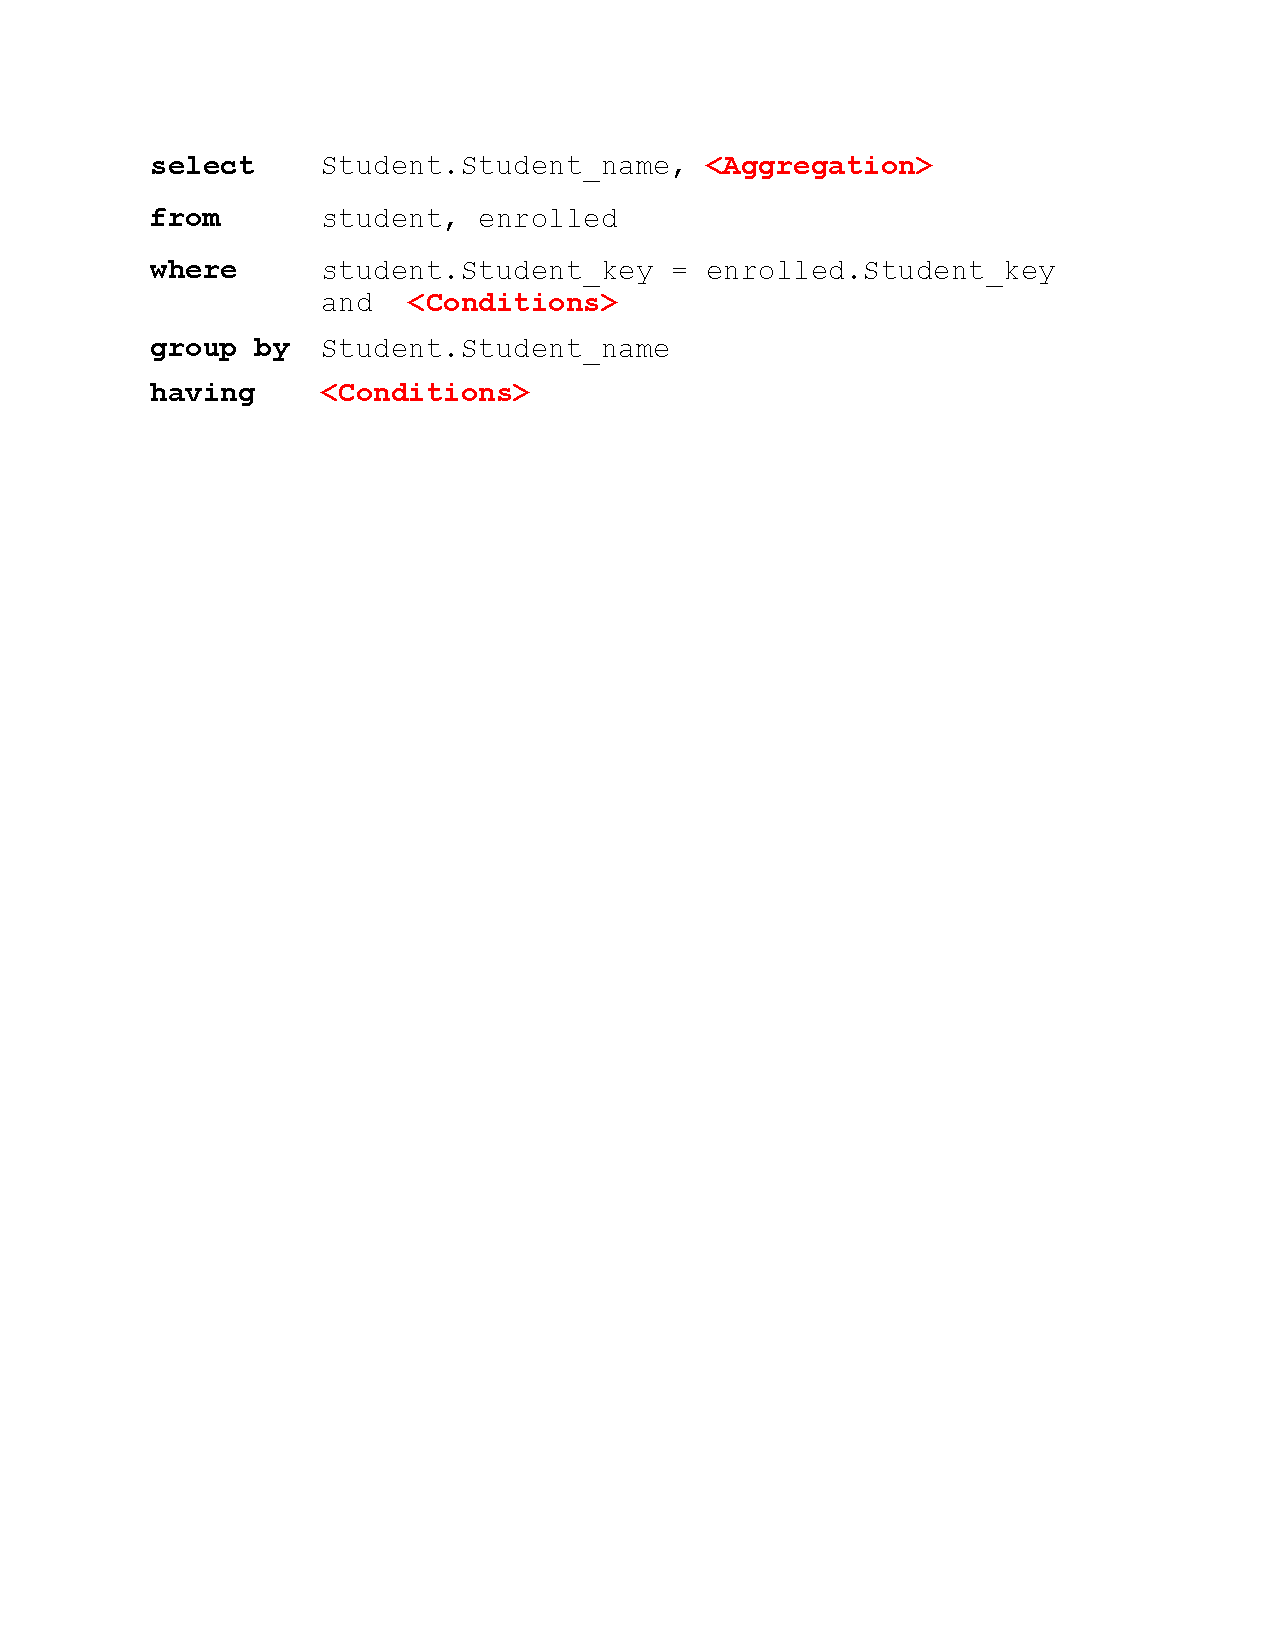
\includegraphics[width=0.45\textwidth]{sql_skeleton.pdf}
	\caption{The SQL skeleton created for the motivating example
in Section~\ref{sec:example}.}
	\label{fig:skeleton}
\end{figure}

The created query skeleton  is shown in Figure \ref{fig:skeleton}.
As we can see from Figure \ref{fig:skeleton},  there are three unknown structures represented
by $<$Aggregation$>$ or $<$Conditions$>$ in red color, which will be filled in the next phase.


\subsection{SQL Query Completion}
\label{sec:completion}

The SQL skeleton produced by the first step, though incomplete,
serves as a good reference in inferring complete and valid SQL queries.
In this step, our technique the remaining incomplete parts: conditions and
aggregates, by rule-based learning and type-directed search, respectively.

\subsubsection{Learning Conditions}
\label{sec:decision_tree}

The problem of learning query \textit{conditions} can be cast as finding
appropriate \textit{rules} that can perfectly divide the whole searching space
into positive part and negative part. In our context, the searching space
contains all tuples generated by joining the input tables, the positive part
are all tuples in the output table, and the negative part are the rest
tuples.

%the rest of tuples. Here our searching space consists of all tuples generated
%by joining input tables. These tuples can be returned by applying our SQL
%skeleton on input database if we remove all holes from the SQL skeleton.

Techniques to efficiently find rules from data has been studied extensively
by many machine learning researchers~\cite{Quinlan:1993, Cohen:1995, Frank:1998}.
Generally, in the machine learning community, there are major two paradigms of
rule learning:

%\begin{itemize}
%\item
\vspace{1mm}
\noindent\textbf{\textit{1. Decision-tree learning~\cite{Quinlan:1993}}}. Given
the positive and negative examples, one can generate a decision
tree, and then extract decision-tree-splitting conditions from the root to
all positive leaf. The extracted conditions can be viewed as the selection
criteria that isolates the output data from the input searching space.


%\item
\vspace{1mm}
\noindent\textbf{\textit{2.``Divide-and-conquer'' strategy~\cite{Pagallo:1990}}}. 
Unlike decision-tree learning, instead of learning a full tree,
this methodology repeatedly determines the most powerful rules for the dataset
that can maximally separate the positive examples from the negative ones, until
no more positive examples are available.

\vspace{1mm}

However, for our problem, both methodologies can not be directly applied.
Learning rules via decision-tree learning is restricted to conjunctive rules,
which is insufficient for many real scenarios. On the
other hand, the generalization ability of the ``divide-and-conquer'' strategy
is quite limited due to overpruning and covering heuristic.

To overcome these two limitations, in our technique, we adapt
the PART learning algorithm~\cite{Frank:1998}, which combines both
rule learning paradigms above. Notably, PART is capable of giving an more
accurate and expressive rule set. Specifically, it utilizes the
``divide-and-conquer'' strategy in that it repeatedly builds rules
and removes the instances it covers until no examples are left.
When creating each rule, it employs a pruned decision tree built from
current set of instance and only makes the leaf with the largest coverage
into the resulting rules, without keeping the whole learned tree in memory.


%In order to use PART, there are two issues that should be considered:

Although PART is a promising algorithm for learning rules from data,
there are two challenges when applying it to our problem:

%We customized PART in the following two aspects to make it applicable
%to our problem:

%\begin{itemize}
%\item
\vspace{1mm}
\noindent {\textbf{\textit{Challenge 1. How to represent tuples.}}}
%the literature of learning from examples~\cite{Mitchell:1997},
In PART, an example data point is represented by a single feature vector.
Therefore, we must transform tuples into appropriate feature representation.
To do so, a straightforward way is simply using concrete values in a tuple
as a feature vector. However, doing so loses much useful structure information
needed in a SQL query.

\vspace{1mm}
%\noindent {\textbf{\textit{Solution 1. Encoding prior knowledge.}}}
We encode existing domain knowledge about SQL query as additional
features, such as, (1) Aggregation, including \CodeIn{COUNT}, \CodeIn{MAX},
\CodeIn{MIN} and \CodeIn{AVG}, whose results might be used in query condition;
and (2) Comparison results between two comparable columns.
The above two additional knowledge encoding permits our technique
to make use of correlations between columns, rather than only values
from each isolated and sequential columns.

%Based on these observations
We add two types of new attributes into feature representation of tuples.

%indicate that not only columns themselves
%are useful for describing a tuple but we also should make use of correlation
%between columns. 

\begin{enumerate}

\item \textit{\textbf{Aggregation Features}}. Aggregation
features are the aggregation results grouped by each \CodeIn{String} type column
over every other columns. Table~\ref{tbl:agg} shows an example.


\item \textit{\textbf{Comparison Features}}. Comparison
feature is the result of comparing two comparable columns. We
consider two possible values:  $\{1, 0\}$,  which represents
means whether two columns under comparison satisfy the predicate or not, respectively.
Table~\ref{tbl:com} shows an example.

%the feature would be $0$. Suppose  the comparison features
%for them are summarized in Table \ref{tbl:com}.

\end{enumerate}

\begin{table}[t]
	\begin{center}
		\begin{tabular}{|c|c|}
		\hline
		\textbf{group by}	& \textbf{aggregation} \\
		\hline
		$C_1$ 				& \textsf{COUNT}($C_2$), \textsf{MAX}($C_3$), \textsf{MIN}($C_3$), \textsf{AVG}($C_3$)\\
		$C_2$ 				& \textsf{COUNT}($C_1$), \textsf{MAX}($C_3$), \textsf{MIN}($C_3$), \textsf{AVG}($C_3$)\\
		\hline
		\end{tabular}
	\end{center}
	\caption{The generated aggregation features for
a table with 3 columns:  $C_1$, $C_2$, and $C_3$, in which
columns $C_1$ and $C_2$ are \textsf{String} type and column $C_3$ is
\textsf{Integer} type.}
	\label{tbl:agg}
\end{table}



\begin{table}[t]
	\begin{center}
		\begin{tabular}{|c|c|}
		\hline
		\textbf{predicate}	& \textbf{comparison result} \\
		\hline
		$C_1=C_2$ 			& 0\\
		$C_1<C_2$ 			& 1\\
		$C_1>C_2$			& 0\\
		\hline
		$C_3=C_4$ 			& 1\\
		$C_3<C_4$ 			& 0\\
		$C_3>C_4$			& 0\\
		\hline
		\end{tabular}
	\end{center}
	\caption{The generated comparison features
for a table with 4 columns: $C_1$, $C_2$, $C_3$,
and $C_4$, in which columns $C_1$ and $C_2$ are \textsf{String} type, and
columns $C_3$ and $C_4$ are \textsf{Integer} type. Columns with
the same type are comparable, such as $C_1$ and $C_2$, and
$C_3$ and $C_4$.
}
	\label{tbl:com}
\end{table}

Combining using concrete tuple values, aggregation
features, and comparison features, our technique is able to
extract expressive feature representation for tuples,
and permits users to encode domain knowledge and structural
information about a SQL query.

%\item
\vspace{1mm}
\noindent {\textit{\textbf{Challenge 2. How to use the learnt rules to complete a SQL query.}}}
PART may return rules including three types of features. For example,
it returns the following rules for our motivating example in Section~\ref{sec:example}:
%. For our
%motivating example there is one rule learned from input tuples. It is

\smallskip
{
\CodeIn{COUNT(enrolled.Course\_key) $>$ 2}
    \CodeIn{\&\& student.level =`senior'}.
}
%\smallskip
\vspace{-2mm}

We need to split the returned rule into two parts: the query selection
condition, and the having condition. To achieve this, we
use $P_o$ to denote predicates related to original features
directly derived by the concrete tuple values,
$P_a$ to denote predicates related to aggregation features and $P_c$ to
denote predicates related to comparison features. For predicate in $P_o$,
we use it to fill condition holes in select clause by comparing selected
column with a constant value. For predicate in $P_a$, we
can use it to fill aggregation holes in having clause.

For our motivating example,
$P_o = \{\CodeIn{student.level =`senior'}\}$, 
$P_a = \{\CodeIn{COUNT(enrolled.Course\_key) $>$ 2}\}$.

After that, our technique adds a having condition such as ``\CodeIn{having COUNT(enrolled.Course\_key)}''
to the SQL query skeleton, and use predicates in $P_c$  to fill the selection condition.
%holes using predicates that compare two columns. There is no such predicate in our motivating example.

%\end{itemize}

\subsubsection{Searching for Aggregates}
\label{sec:agg_search}

The last step in completing a SQL query is searching for aggregates as the projection
columns. Our technique uses a type-directed searching strategy to do this. The whole
searching space includes all possible combinations of table columns and the five supported
aggregates (see Figure~\ref{fig:syntax}). In type-directed search, we leverage the following
information to prune the potential space:

\begin{enumerate}
\item The output values' type in the result column must be compatible with the aggregate's return
type. For instance, if an output column is String type, it must not use aggregates that always
return an Integer type, such as \CodeIn{count} and \CodeIn{sum}.

\item When using arithmetic aggregates such as \CodeIn{max} and \CodeIn{min}, the values
in the output column must have appeared in the input table.
\end{enumerate}

In our experience, the type-directed searching strategy significantly reduces the
searching space and makes our tool find the desirable aggregates faster.


\subsection{Query Candidate Ranking}
\label{sec:ranking}

After the above two steps, SQL queries satisfying the given input-output examples
will be returned. To reduce the effort in inspecting the
results and selecting a desirable query, we devise a strategy
to put the most likely query near the top of the return list.
%Due to lacking in input-output examples we are not be able to rule out SQL
%queries that lack in generalization ability. Instead we will provide user queries according to a rank.

Our strategy is based on Occam's razor to
compute a cost for each returned query, and prefers
queries with lower costs.
%queries in the increasing order of their costs.
For a SQL query, each table appearing in it introduces a cost $C_t$ and each appearing condition 
introduces an additional cost $C_p$. The total cost of a query is
computed by: $n_t \cdot C_t+n_p \cdot C_p$, where
$n_t$ is the number of tables and $n_p$ is the number of predicates used in the query. Our technique 
ranks queries based on their costs in an increasing order to ensure that a simpler query often ranks higher.
Figure~\ref{fig:rank} shows an example to illustrate this ranking strategy.


\begin{figure}[t]

\centering
\begin{tabular}{|l|l|}
%\hline
\multicolumn{2}{l}{Input table: \textbf{student}}\\\hline
%\hline
\textbf{name} & \textbf{score} \\\hline
Bob & 4  \\\hline
Dan & 5  \\\hline
Jim & 2  \\\hline
\end{tabular}
\quad
\begin{tabular}{|l|}
%\hline
\multicolumn{1}{l}{Query output}\\\hline
%\hline
\textbf{name}\\\hline
Bob  \\\hline
Dan  \\\hline
\end{tabular}

\vspace{2mm}


Query 1:
\vspace{-4mm}
\begin{CodeOut}
\begin{alltt}
\centering
\textbf{select name from student where score > 3;}
\end{alltt}
\end{CodeOut}

Query 2:
\vspace{-4mm}
\begin{CodeOut}
\begin{alltt}
\centering
\textbf{select name from student where name = `Bob` or name = `Dan`
}
\end{alltt}
\end{CodeOut}
\vspace{-5mm}
\Caption{{\label{fig:rank} The illustration of our query candidate ranking
strategy. Both Query 1 and Query 2 can transform the example input
to the example output. However, based on our ranking strategy, Query 1
is ranked higher, since it contains less conditions and is simpler
than Query 2.
An inferred query containing more conditions like Query 2 is more likely
to overfit the given examples.}}
\end{figure}



%\subsection{User Interactive Model}
%\label{sec:uim}




%
\section{Implementation}
\label{sec:implementation}




\pagebreak


\section{Evaluation}
\label{sec:evaluation}

We implemented our technique in an open-source programming tool.
Our tool employs WEKA \cite{Hall:2009} to implement the PART learning algorithm
 to extract rules, and uses MySQL~\cite{mysql} as the backend database engine
to check the validity of each output query.
When a SQL query is synthesized,
our tool executes the synthesized query on the backend database,
and checks whether the output query result matches the given example output.

We next describe the evaluation of our prototype tool.

\subsection{Research Questions}

We aim to investigate the following research questions:

\begin{itemize}
\item Is the supported SQL subset expressive enough to describe
queries that real end-users require?

\item Can our technique efficiently find a SQL query
from small input-output examples?

%\item Does the inferred SQL query correctly express end-users'
%intention and produce the expected output? If not, how many
%additional examples does a user need to provide before our
%approach infers a correctly-behaved SQL query?

\end{itemize}


\subsection{SQL Query Synthesis Scenarios}

To answer these two questions, we collected a set
of SQL query synthesis scenarios in the following
two ways. First, we picked
up 6 SQL exercises from a classic database textbook~\cite{cowbook}.
Those 6 SQL exercises cover many commonly-used SQL features,
which a database course instructor think would be the most useful parts,
and expect her students to get familiar with. Second, we collected
5 SQL problems raised by real end-users from popular online help forums
~\cite{stackoverflow, tutorialized, dbjournal}.

%evaluation
%subjects from two major sources: exercises from classic
%database textbooks like, and real-world questions
%that end-user asked on well-known online help forums. Specifically,
%we aim to apply our implemented tool solve SQL query related questions
%after Chapter 3 (SQL DML) in~\cite{cowbook}. We have also collected
%19 end-user questions from online forums, and plan to apply our
%tool to solve them.

For a given exercise or problem, if it
has already been associated with input-output examples (e.g.,
those provided by users from online forums),
we directly apply our tool on the existing examples.
Otherwise, we manually provide small concise and representative
input-output examples for our tool.
If for a given exercise or problem, our tool inferred
a SQL query that does not behave as we expected when applied
to other inputs, we will manually find an input on which the
SQL query misbehaves and reapplied our tool to the new input. We
repeat this process until our tool infers a desirable SQL query.

\subsection{Experimental Results}

\begin{table}[t]
\setlength{\tabcolsep}{.14\tabcolsep}
\begin{tabular}{|c|c|c|c|c|}
\hline
 & \#Total& \#Solved& Time Cost (s) & Human Effort (m)\\
 \hline
 Textbook exercises &  6 &  5 &  30 & 3 \\
\hline
 Forum problems &  5 &  5  &  60 & 5\\
\hline
\end{tabular}

\Caption{{\label{tab:results} Experimental results of synthesizing
SQL queries for 6 exercises from a classic database textbook~\cite{cowbook},
and 5 real problems from online forums. Column `\#Total' is the total
number of exercises or problems used in the experiments. Column
`\#Solved' is the number of solved
exercises or problems by our technique. Column `Time Cost(s)'
records the average time (in seconds) used to solve each exercise or problem.
Column `Human Effort(m)' is the average time (in minutes) spent in
preparing input-output examples for each exercise or problem without
existing examples.}}
\end{table}

For each SQL synthesis scenario, we measured two results.
The time cost in producing
a desirable SQL query by our tool, and
the time we spent in writing input-output examples.
%For each exercise or problem, we also record
%how much time we spent in writing input-output examples.
Table~\ref{tab:results} summarizes our experimental results.

As shown in Table~\ref{tab:results}, our technique synthesized
expected SQL queries for 10 out of 11 scenarios
within a very small amount of time (less than 1 minute each).
The human effort spent in providing input-output examples
is also very limited: it took us less than 5 minutes for one scenario.
%per exercise (or problem).


\subsubsection{A Real Example}
We next describe a real SQL problem picked up from
an online SQL help forum\footnote{\url{http://forums.tutorialized.com/sql-basics-113/join-problem-147856.html}}.
The thread was started by a novice user, who needed help to write a
SQL query to get result from three input tables. In the help thread, the
novice user described his required query in a few paragraphs of
English, but also include several small, representative input-output
examples as shown in Figure~\ref{fig:example}, to better express
his intention. 
This thread receives no replies as of May 2012, and we speculated that
writing a SQL query to join three tables to produce certain output results
can be non-trivial.

We ran our tool on the input-output examples
in Figure~\ref{fig:example}. The tool produced 6 valid answers
in less than 1 minutes, all of which satisfy the given examples. The
highest ranked SQL query is shown in Figure~\ref{fig:answer},
which is quite unintuitive to write. The SQL query in Figure~\ref{fig:answer}
first joins three input tables
on columns \CodeIn{T1.Column2}, \CodeIn{T2.Column2},
\CodeIn{T2.Column1}, and \CodeIn{T3.Column1} using some
selected columns, and then aggregates the results based on
column \CodeIn{Table2.Column3}'s value. Finally, it
returns the minimal values of columns \CodeIn{T1.Column1}, \CodeIn{T1.Column4}, and \CodeIn{T3.Column2}
from each aggregated group as the results.

%Such help threads on online discussion forums are not rare, but the SQL
%queries needed to address them are non-trivial.

\begin{figure}[t]
\centering
\textbf{The input Table1:}

\begin{tabular}{|c|c|c|c|}
\hline
 Column1 & Column2& Column3& Column4\\
 \hline
 101 &  2001 &  3020 &  01-01-11\\
\hline
 101 &  2001 &  3002 &  02-01-11\\
\hline
 101 &  2001 &  3001 &  03-01-11\\
\hline
 102 &  2002 &  3002 &  01-01-11\\
\hline
\end{tabular}

\vspace{2mm}

\textbf{The input Table2:}

\begin{tabular}{|c|c|c|}
\hline
 Column1 & Column2& Column3 \\
 \hline
 20011 &  2001 &  200131\\
\hline
 20012 &  2001 &  200132\\
\hline
 20013 &  2001 &  200133\\
\hline
\end{tabular}

\vspace{2mm}

\textbf{The input Table3:}

\begin{tabular}{|c|c|}
\hline
 Column1 & Column2\\
 \hline
 20011 &  Site\\
\hline
 20012 &  Site\\
\hline
 20013 &  Site\\
\hline
\end{tabular}

\vspace{3mm}

\textbf{The output table:}

\begin{tabular}{|c|c|c|c|}
\hline
 101 & 200131 & 01-01-11 & Site\\
 \hline
 101 & 200132 & 01-01-11 & Site\\
 \hline
 101 & 200133 & 01-01-11 & Site\\
 \hline
\end{tabular}
\Caption{{\label{fig:example} Input-output examples taken from
an online SQL help forum thread. Our technique 
automatically synthesizes a SQL query as shown in Figure~\ref{fig:answer}
that produces the output table from the three input tables.
}} \vspace{2mm}
\end{figure}

\begin{figure}[t]
\begin{CodeOut}
\begin{alltt}
\textbf{select min(T1.Column1), T2.Column3,
       min(T1.Column4), min(T3.Column2)
from Table1 T1, Table2 T2, Table3 T3
where T1.Column2 = T2.Column2 and T2.Column1 = T3.Column1
group by T2.Column3}
\end{alltt}
\end{CodeOut}
\vspace{-5mm}
\Caption{{\label{fig:answer} The highest ranked SQL query inferred
by our technique from the input-output examples in Figure~\ref{fig:example}.}}
\end{figure}


\subsection{Experimental Conclusions}

Our initial experimental results are promising.
It shows that the supported SQL subset is
expressive enough to describe a variety of useful database queries.
It also demonstrates the usefulness of our SQL query
synthesis technique.  In particular, our SQL query synthesis technique only requires a small amount of
human effort and small input-output examples. It infers 
desirable SQL queries on both database textbook exercises
and online forum problems, even solving problems that receive no reply
from popular online forums.







\section{Related Work}
\label{sec:related}

Our work can be differentiated from existing work in three major ways: the scope
of the problem addressed, the technique used, and the evaluation methodology.
We next discuss two categories of closely-related work on reverse query processing
and automated program synthesis.


\subsection{Reverse Query Processing}

In the database community, there is a rich body of
work~\cite{Zloof:1975, Tran:2009, DasSarma:2010} that share the same broad principle
of ``reverse query processing''. Zloof's work on \textit{Query by Example} (QBE)
~\cite{Zloof:1975} provided an intuitive form-based Graphical User Interface for
writing database queries, which is completely different than ours.

The problem of \textit{Query By Output} (QBO)~\cite{Tran:2009} shares a similar
goal with QBE, but takes a quite different approach.
In QBO, we are given a view: $V$ and $n$ relations: $R_1, R_2, ..., R_n$ and asked to
return a query $Q$ such that $Q(R_1, R_2, ..., R_n)$ = $V$. However, QBO is cast as
a classification problem (into two classes: tuples in $V$, and tuples not in $V$)
and decision trees are used to find a compact query. A decision tree is constructed
in a greedy fashion by determining a ``good'' predicate to split the tuples into two
classes, which form the root nodes of two decisions trees (each of which is
constructed in a recursive fashion).  The QBO technique presented in~\cite{Tran:2009}
infers select-project-join queries. Such queries can only be applied to
satisfy a limited number of examples, and cannot be applied to many of the other
real world cases that we studied (e.g., a query with an aggregation operator
like our motivating example in Figure~\ref{fig:example}).

Recently, the \textit{View Definitions Problem} (VDP) has been addressed
by Sarma et al.~\cite{DasSarma:2010}.
VDP is restricted to find the most succinct and accurate view definition, when
the view query is restricted to a specific family of queries. VDP is the special
case of QBO where $n = 1$ and there are no joins nor projections.
The high-level goal of this work is similar to our approach, but there
are some key differences: (1) VDP techniques infer a relation from a large representative
example view, while we infer a SQL query from a set of few input-output examples
(which is a critical usability aspect for end-users who lack adequate
SQL experience). (2) the VDP technique in~\cite{DasSarma:2010} does
not consider join or projection
operations and assumes the output view to be a strict subset of the input
database with the same schema, while our work considers both join and
projection operations.


In the data mining community, a slightly related problem to ours is
the \textit{redescription mining} problem~\cite{Ramakrishnan:2004}.
At an abstract level, our work is different from these redescription mining
techniques in several ways.
First, the goal of redescription mining is to find different subsets of
data that afford multiple descriptions across multiple vocabularies
covering the same dataset, while our goal is to infer a SQL statement
to obtain the desirable querying behavior.
Second, we are concerned with a fixed subset of the data (i.e., the output example table).
Third, none of the existing approaches for redescription mining account for
structural (relational) information in the data. 

Other query recommendation systems proposed in the literature may achieve
a similar goal of helping end-users write better SQL queries, but they rely on information
that we cannot assume access to in many realistic scenarios: a query log~\cite{Khoussainova:2010},
or user history and preferences~\cite{Howe:2011}.

\subsection{Automated Program Synthesis }

Program synthesis is the problem of creating a program
in some underlying language from specifications that can range
from logical declarative specifications to examples or
demonstrations~\cite{Harris:2011, singh:2012, Gulwani:2011}.
This topic has been studied intensively in Artificial Intelligence and
Programming Language communities with the goal of easing the burden of
algorithm designers, software developers, or end-users.
Interest in it has grown rapidly in recent years~\cite{Gulwani:2010:DPS},
and many approaches have been proposed.

Example-based program synthesis techniques~\cite{Kandel:2011, Fisher:2008,
Fisher08Pads,Lau:2003:PDU, Lau:2000:VSA, Barbosa:2010:MLA, Arasu:2009:LST}
take textual input-output examples and infer programs that transform text.
However, existing techniques focused on synthesizing programs for string
expressions~\cite{singh:2012, Gulwani:2011}, spreadsheet layout transformation~\cite{Harris:2011},
, geometry constructions~\cite{Gulwani:2011:SGC}, thus
can not be directly applied to our SQL query synthesis domain,
due to different abstractions, granularities, and tasks.



\section{Conclusions and Future Work}
\label{sec:conclusion}

General purpose programming platforms have never been easy. Many end-users
who are non-professional programmers are still mostly stucked with the process
of \textit{how} to accomplish a certain task by receiving 
step-by-step, detailed, and syntactically correct instructions, instead of simply describing
\textit{what} the task is. \textit{Programming by examples} has the potential
to change this landscape, when targeted for the right set of people for the
right set of problems.

In this paper, we studied the problem of automated SQL query synthesis
from simple input-output examples, presented a practical technique to 
infer desirable SQL queries that fulfill end-users' intentions, and
developed a usable programming tool.
To demonstrate usefulness of our technique, we applied our tool
to 6 SQL exercises from a classic database textbook as well as
5 non-trivial SQL problems from online forums by real end-users. 
The results are promising, showing that our technique can automate a variety of database
query tasks.

The source code of our tool implementation is available at: \\
\url{http://sqlsynthesizer.googlecode.com}

\vspace{1mm}

Besides general issues such as performance and ease of use, our future
work will concentrate on the following topics:

\textbf{Enrich the supported SQL subset.} The technique 
presented in this paper focuses on a widely-used SQL subset.
It may miss some important language features such as
nested queries, and thus fail to infer meaningful queries
in some scenarios when such missing features must be used.
We plan to remedy this problem by enriching the
supported SQL subset, and designing a corresponding algorithm
to synthesize more general solutions.

\textbf{Illustration of the synthesis steps.} Besides
producing a final result, end-users may also be interested in knowing
how a SQL query is inferred.  Showing detailed inference steps (visually) not
only makes the tool more usable, but only permits
end-users to better understand the whole process and spot possible errors earlier.
To do so, we plan to investigate how to apply recent advance in data
visualization~\cite{Kandel:2011}
to the context of program synthesis.

\textbf{Noise detection and tolerance in users' inputs.} The current technique
requires users to provide noise-free input-output examples.
Even in the presence of a small amount of user-input noises (e.g., a typo),
the inference algorithm will declare failure when it fails to learn
a valid SQL query.
To overcome this limitation, we plan to design a more robust inference
algorithm that can attempt to identify and tolerate user-input noises,
and even suggest a fix to the noisy example.



\textbf{Generalization.}
We have applied our synthesis technique to one specific, but
important problem.  There is a rich history of end-user programming
problems being cast as program synthesis (e.g.,~\cite{Gulwani:2010:DPS}).  In future
work, we plan to formulate other tasks, such as repetitive file operations, and to apply our technique to them.





\vspace{2mm}

%\noindent \textbf{Acknowledgement.} We would like
%to thank Stephen Fink and Manu Sridharan for
%answering our questions about WALA.
%\vspace{-2mm}

\bibliographystyle{abbrv}
\small{
\bibliography{sqlsynthesis}
}
\end{document}
